\documentclass[10pt,a4paper]{article}

\usepackage{fontspec}
\usepackage[top=1cm]{geometry}
\usepackage[backend=bibtex]{biblatex}
\usepackage{hyperref}
\usepackage{graphicx}
\usepackage{subfig}
\defaultfontfeatures{Mapping=tex-text}
\setromanfont[Ligatures={Common},Numbers={Lining}]{Linux Libertine}
\author{Michal Staniaszek}
\title{Thesis Literature Review}

\bibliography{../report/report.bib}

\begin{document}
\maketitle
\section{Segmentation}
Popularised by Comaniciu~\cite{comaniciu2002mean} for use in image segmentation,
mean shift was first introduced by Fukunaga~\cite{fukunaga1975estimation} in
1975, and rediscovered by Cheng~\cite{cheng1995mean} in 1995. The technique finds
stationary points in a density estimate of the feature space, for example pixel
RGB values, and uses those points to define regions in the space by allocating
pixels to them. Pixels which follow the gradient of the density to the same
stationary point are part of the same segment. An example can be seen in
Figure~\ref{fig:meanshift}.
\begin{figure}[t]
  \centering
  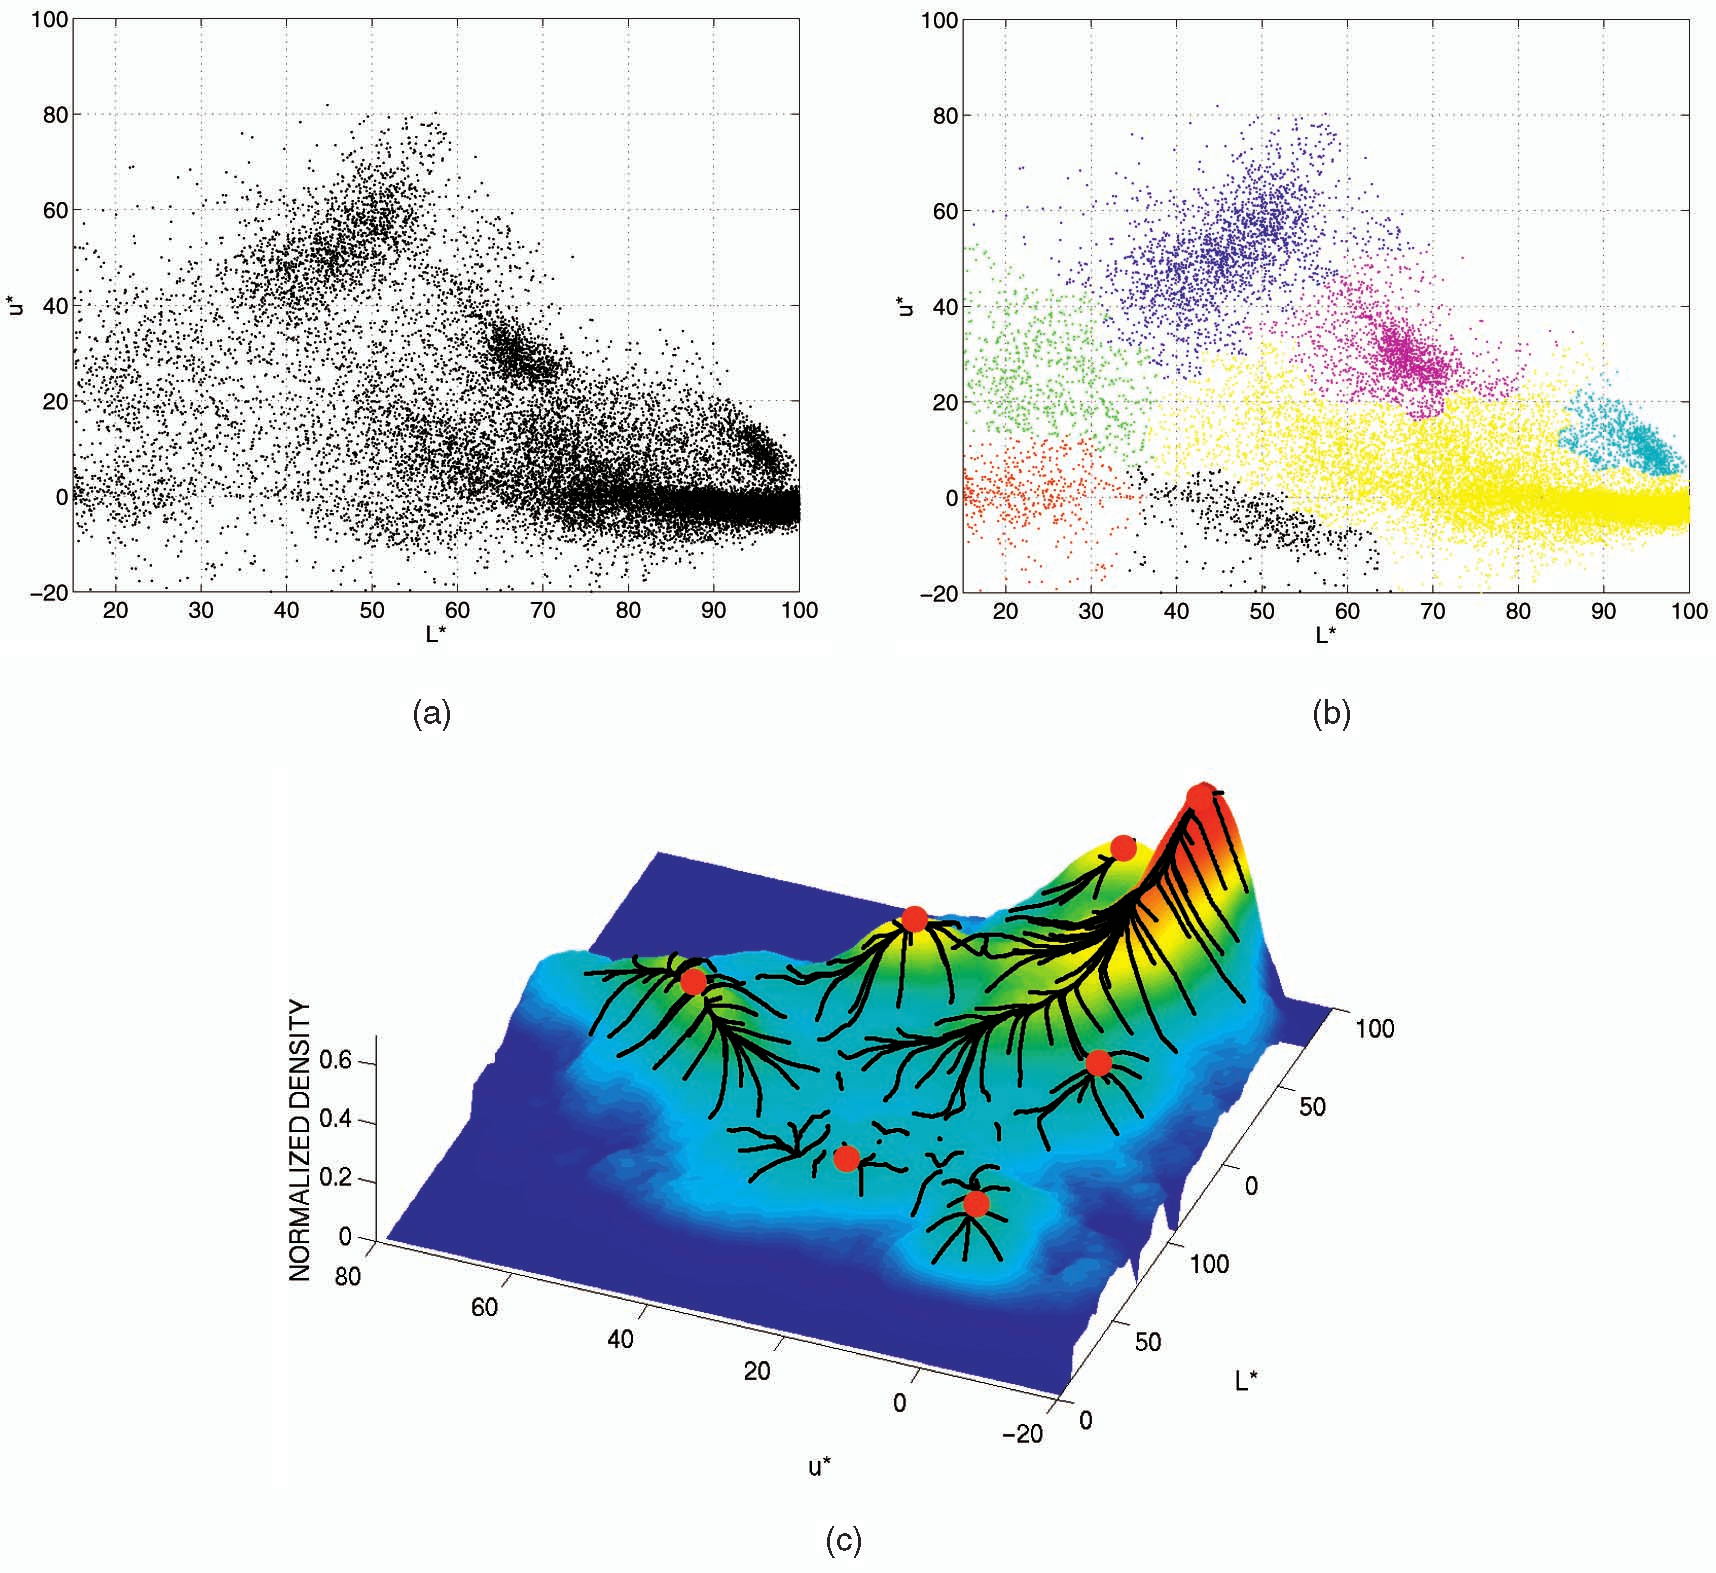
\includegraphics[width=\textwidth]{images/meanshift}
  \caption{Visualisation of mean shift \cite{comaniciu2002mean}. a) First two
    components of image pixels in LUV space. b) Decomposition found by running
    mean shift. c) Trajectories of mean shift over the density estimate.}
  \label{fig:meanshift}
\end{figure}
\section{Interest Points}
Mikolajczyk and Schmid~\cite{mikolajczyk2004scale} introduce an interest point
detector which is an improvement on SIFT \cite{lowe2004distinctive} and the
Laplacian of Gaussians \cite{lindeberg1998feature} in the sense that it is able
to deal with affine transformations. They do not, however, introduce a new type
of descriptor to go with the point selection.
\section{2D Descriptors}
Different considerations must be made for 2D images because of affine
transforms, rotation and so on

Van Gool \cite{van1996affine} gives a description of how to use moment
invariants to recognise planar patterns like labels and signs under affine
deformations. The moments describe things like the size of the shape and its centre
of mass, or statistics like the mean and variance of pixel intensities in the
shape. These moments can be combined in such a way that they are invariant to
deformations, which is useful to have in a descriptor.
\section{3D Descriptors}
The Ensemble of Shape Functions (ESF) descriptor introduced in
\cite{wohlkinger2011ensemble} by Wohlkinger and Vincze combines the Shape
Distribution approach introduced by \cite{osada2002shape} along with some
extensions proposed in \cite{ip2002using}. It also makes use of their
voxel-based distance measure from \cite{wohlkinger2011shapedist}. Pairs or triples of
points are sampled from segmented partial clouds of objects, and histograms are
created by extracting information such as distance, angle, ratios, and whether
points are inside or outside (or a mix) of the model. See
Figure~\ref{fig:wohlESF}.

The Point Feature Histogram (PFH) was introduced by Rusu et al. in
\cite{rusu2008persistent}. It creates descriptors based on the angles between a
point on a surface and $k$ points close to it. The Fast Point Feature Histogram
(FPFH) improved the speed of computation, and allowed the use of the descriptor
in real time \cite{rusu2009fast}. The Viewpoint Feature Histogram (VFH) extended
the FPFH by adding viewpoint information to the histogram by computing
statistics of surface normals relative to the viewpoint \cite{rusu2010fast}. It
also improved the speed of the FPFH. The clustered version (CVFH) further
improved the viewpoint technique by mitigating the effect of missing
parts and extending it to be able to estimate rotations of objects
\cite{aldoma2011cad}.

Multi-scale descriptors are useful as they can be used to characterise regions
of varying size. Cipriano et al. introduce such a descriptor for use on meshes
\cite{cipriano2009multi}. It captures the statistics of the shape of the
neighbourhood of a vertex by fitting a quadratic surface to it. Vertices in the
region are weighted based on distance from an initial vertex, and a plane is
constructed using a weighted average of the face normals. The parameters of the
quadratic are then used to find its principle curvatures, which make up the
descriptor.

Work in protein-protein docking also uses 3D descriptors to help with
simulations of an otherwise lengthy and complex process. The Surface Histogram
is introduced by Gu et al. \cite{gu2012surface}, and uses the local geometry
around two points with specific normals on the surface of a protein. A
coordinate system is defined by the two points and the line between them, and a
rectangular voxel grid is defined around the points. The grid is then marked in
locations where the surface crosses the grid, and a 2D image is constructed by
squashing the data onto one of the axes. The descriptor is designed to
immediately give a potential pose for the docking.

Another example of a shape descriptor from biology is the Context Shape
\cite{shentu2008context}. A sphere is centred on a point, and rays are projected
from this point to points evenly distributed on the surface of the sphere. Each
of the rays is divided into segments, with a binary value associated with each
segment depending on whether the segment is inside or outside the protein. To
compare the descriptor, a rotation is applied to match the rays, and a volume of
overlap is computed based on matching bits in the rays.
 
\begin{figure}
  \centering
  \subfloat[]{
    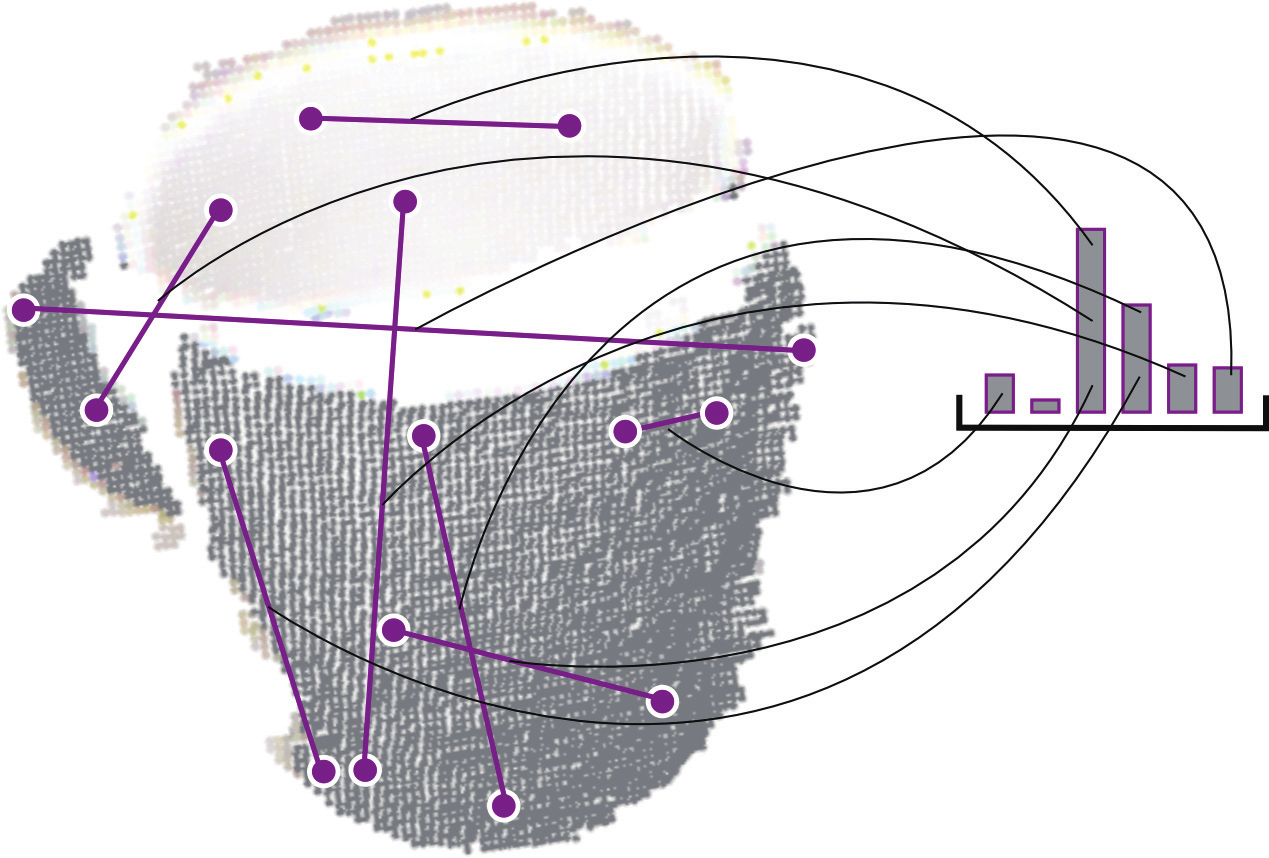
\includegraphics[width=0.23\textwidth]{images/wohl_d2}
  }
  \subfloat[]{
    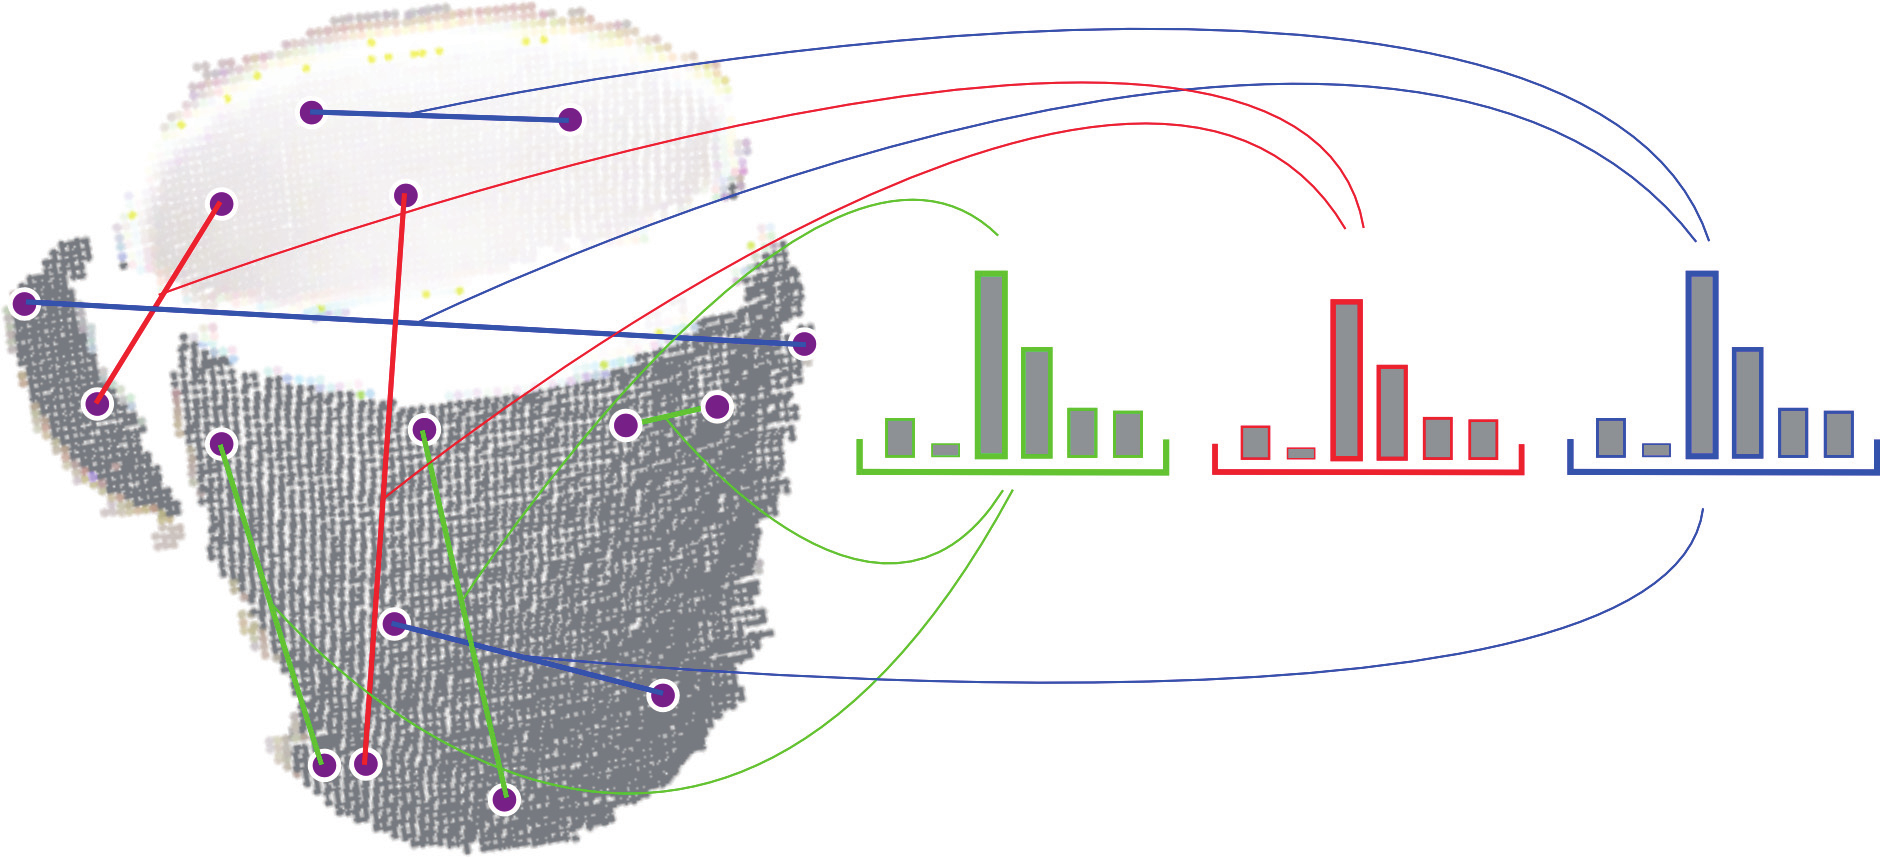
\includegraphics[width=0.23\textwidth]{images/wohl_onoff}
  }
  \subfloat[]{
    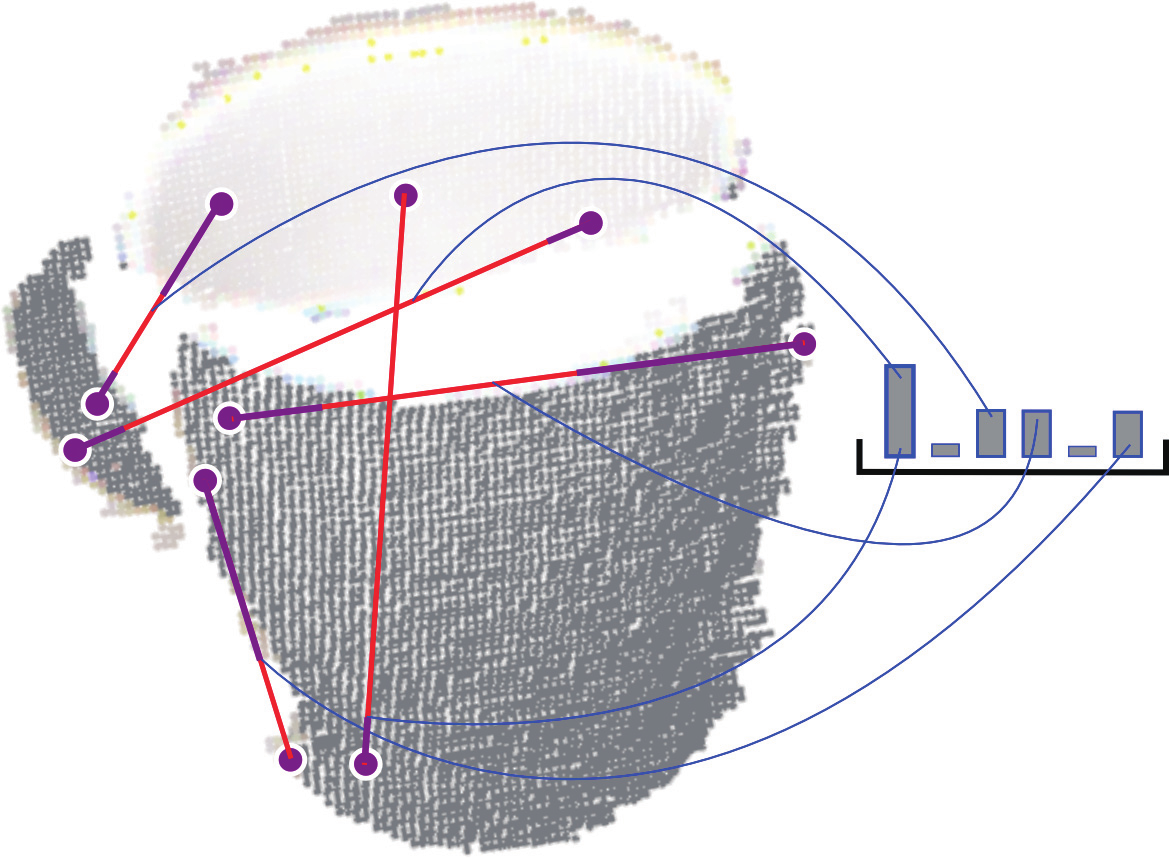
\includegraphics[width=0.23\textwidth]{images/wohl_ratio}
  }
  \subfloat[]{
    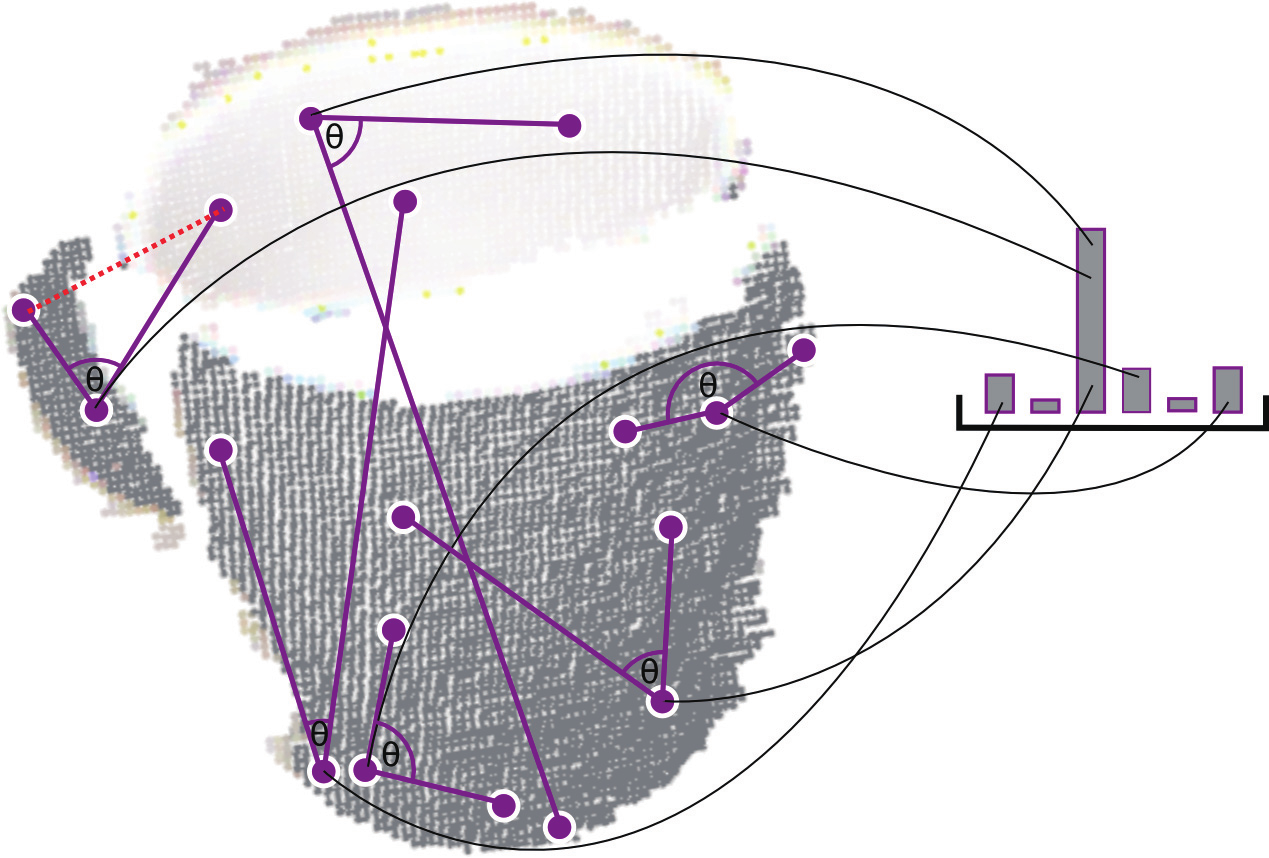
\includegraphics[width=0.23\textwidth]{images/wohl_a3}
  }
  \caption{Examples of the measures used to construct the Ensemble of Shape
    Functions histograms of \cite{wohlkinger2011ensemble}. a) Distance between
    points. b) Whether the points are on or off the model, or mixed. c) Ratio of
  line segments on and off the surface of the model. d) Angle between pairs of lines.}
  \label{fig:wohlESF}
\end{figure}

The splash descriptor was introduced by Stein et al. \cite{stein1992structural}.
A point on the surface with a given surface normal (the reference normal) is
chosen, and a slice around that with some geodesic radius (distance along the
surface) is computed. Points on the circle are selected using some angle step,
and the normal at that point is determined. A super splash is when this process
is repeated for several different radii. For each normal on the circle,
additional angles between it and a coordinate system centred on the reference
normal are computed. These angles and the angle around the circle are then
mapped into a 3D space, where polygonal approximation is made, connecting each
point with a straight line. Some additional computation is done to allow the
encoded polygons to act as a hash. The method is quite complex.

\begin{figure}
  \centering
  \subfloat[]{
    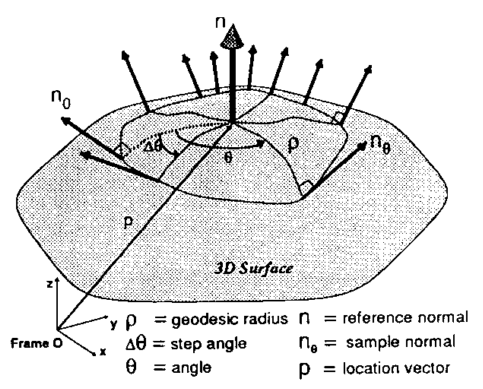
\includegraphics[width=0.32\textwidth]{images/splash}
  }
  \subfloat[]{
    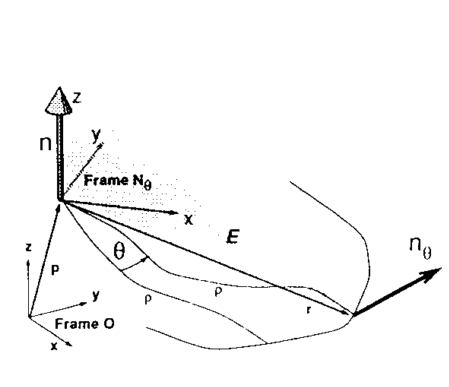
\includegraphics[width=0.32\textwidth]{images/splash_normals}
  }
  \subfloat[]{
    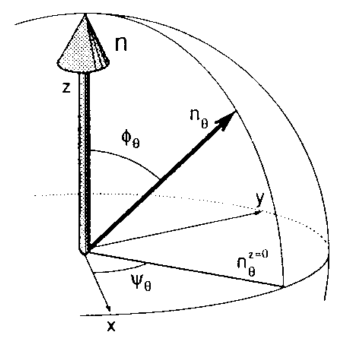
\includegraphics[width=0.32\textwidth]{images/splash_angles}
  }
  \caption{Splash descriptor \cite{stein1992structural}. a) shows the splash and
    normals around it. b) and c) show how the additional angles are defined.
  }
  \label{fig:splash}
\end{figure}

Point Signatures are similar to the splash descriptor in the sense that they
both sample points on a circle \cite{chua1997point}. This descriptor again
selects a reference normal, and has a specific radius. This time, the radius
defines a sphere around the point. The intersection of the surface with the
sphere is a 3D space curve. The orientation of the curve is defined by fitting a
plane to it. The distances between the space curve and the fitted plane at
sampled points define the signature of the reference point. These signatures can
be compared by lining them up and checking whether the query falls within the
tolerance band of previous signatures.

\begin{figure}
  \centering
  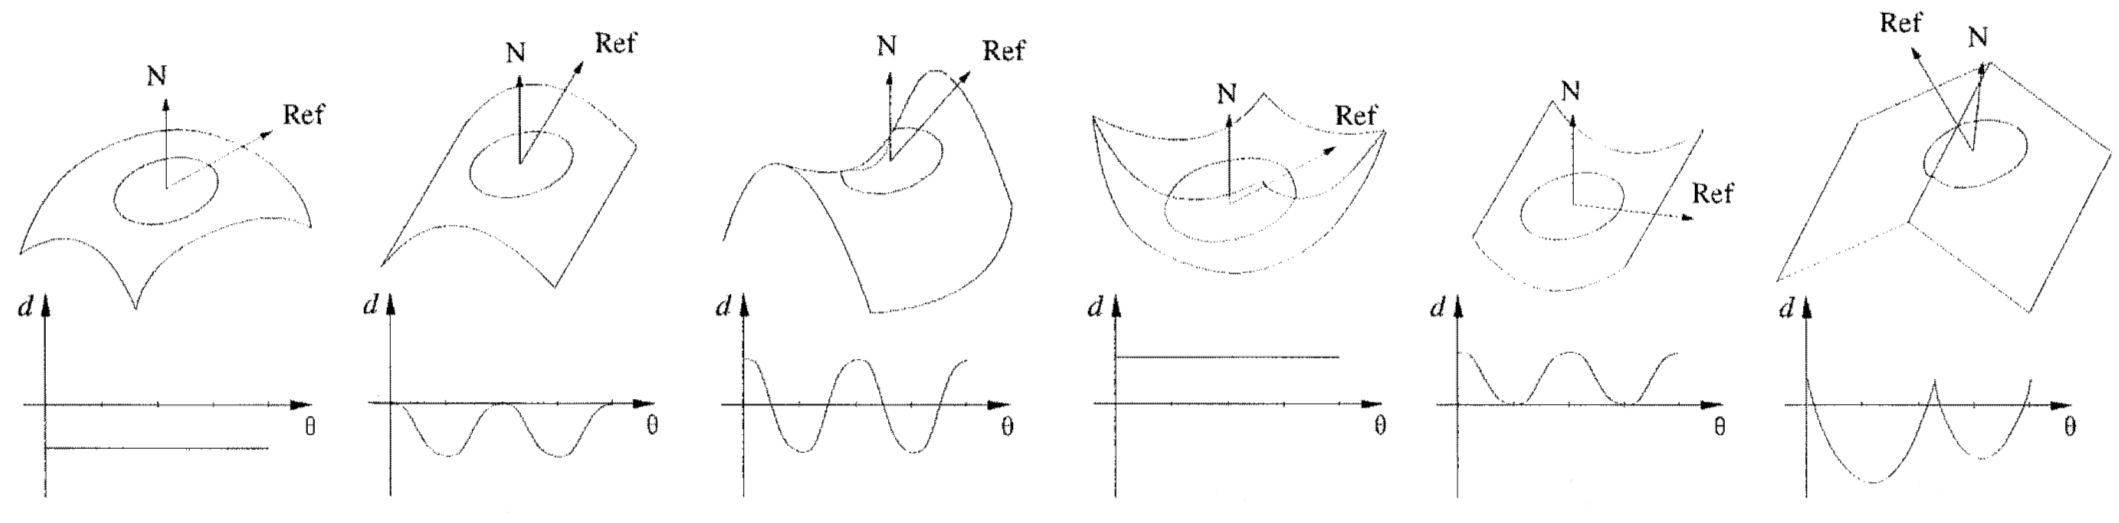
\includegraphics[width=\textwidth]{images/pointsig}
  \caption{Examples of the point signature responses to different surfaces
    \cite{chua1997point}. $d$ is the distance from the reference vector to the
    space curve defined by the intersection of the surface with a sphere centred
    at $N$. Ref rotates about $N$.}
  \label{fig:pointsig}
\end{figure}
\section{Point Matching}
In \cite{chui2003new}, Chui and Rangarajan introduce an extension to ICP which
allows for non-rigid registration and improved robustness to outliers. In
contrast to ICP, their approach does not use the nearest-neighbour approach to
define correspondence. Instead, they use an alternating algorithm similar to
expectation maximisation. Annealing is used to prevent binary correspondences
when the algorithm is not yet close to the solution --- at the beginning there
is a large search range for correspondences, which gradually shrinks as the
temperature decreases.
\section{Model Matching}
\begin{figure}
  \centering
  \subfloat[Conformal factors. High value indicates high required deformation to
  sphere \cite{ben2008characterizing}.]{
    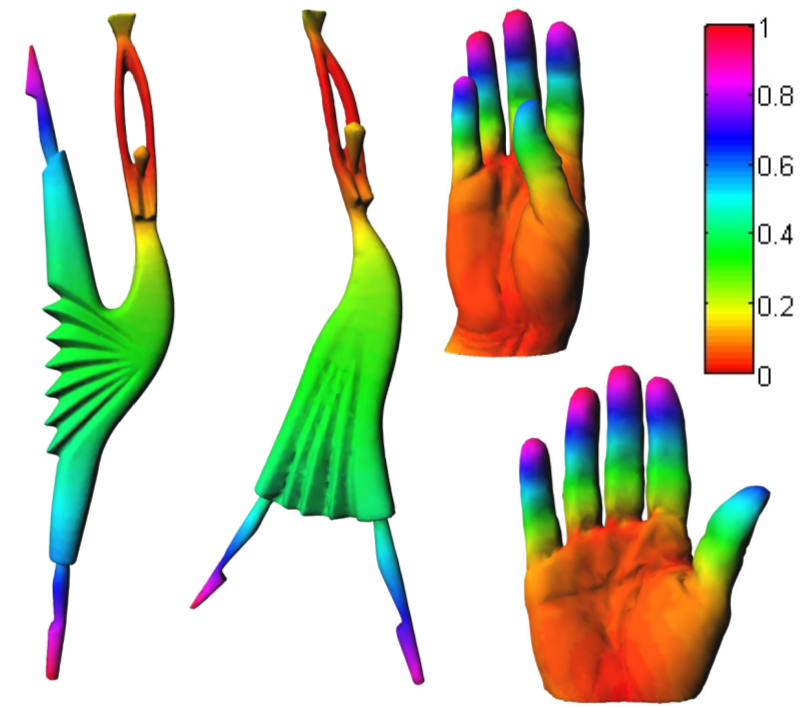
\includegraphics[width=0.48\textwidth]{images/conformal.png}
    \label{fig:conform}
  }
  \caption{Model matching approaches}
  \label{fig:modelmatch}
\end{figure}
In \cite{ben2008characterizing}, Chen et al. describe another approach to model
matching using conformal factors. This technique uses ideas from conformal
geometry, transforming the mesh of an object such that it has a uniform Gaussian
curvature. Information is stored about how much deformation is needed locally to
globally transform the object into a sphere --- this is the conformal factor.
The factor is based on a global computation on the whole mesh, as opposed to
per-vertex computations of the Gaussian curvature, which makes it much smoother
and appropriate for use in histograms. The histogram of a sample of the factors
is used as a descriptor, and is pose invariant, as seen in
Figure~\ref{fig:conform}. The authors say that it should be possible to use the
approach in partial model matching.
\section{Storing and Querying Descriptors}
There are several techniques for storing and querying descriptors, mostly based
on some form of tree. Recently, the k-d tree\cite{bentley1975multidimensional,
  friedman1977algorithm} has been used for efficient approximate matching with
either an error bound \cite{arya1998optimal}, where there is a bound placed on
the error between the true nearest neighbour and the one found, or a time bound
\cite{beis1997shape}, where the search is stopped after examining a certain
number of leaf nodes. Further improvements on the k-d tree are introduced in
\cite{silpa2008optimised}, where multiple randomised trees are used to optimise
the search. A priority search tree algorithm is introduced in
\cite{muja2014scalable}, which appears to be very effective. This may be the
same one as in \cite{muja2009fast}. The algorithm in the last two papers has
been integrated into PCL, which is useful.

The vocabulary tree \cite{nister2006scalable} makes use of techniques from
document search to index images. Using $k$-means clustering, construction stage
creates a hierarchical quantisation of the image patch descriptors. In the query
phase, descriptors are compared to the cluster centres, and go down the tree
until a leaf is reached. The path through the tree is used as a scoring measure
to present retrieval results.

Philbin et al. \cite{philbin2007object} show that flat (single-level) $k$-means
clustering can be scaled to large vocabulary sizes if approximate nearest
neighbour methods are used. Early systems for image retrieval used a flat
clustering scheme, which could not scale to large vocabularies
\cite{sivic2003video}. The paper also introduces a re-ranking method which uses
spatial correspondences, which improves the retrieval quality.

Boiman et al. \cite{boiman2008defense} introduce the Naive Bayes Nearest
Neighbour (NBNN) classifier, which seems to be quite relevant. It uses nearest
neighbour distances in the space of descriptors instead of images, computing
``image-to-class'' distances without quantising the descriptors. In general,
quantisation allows for dimensionality reduction, at the expense of the
discriminative power of descriptors. NBNN ``can exploit the discriminative power
of both (few) high and (many) low informative descriptors''. The problem here is
that the classes must be known beforehand, and in our case we do not have that
information. The local NBNN \cite{mccann2012local} does not do the search based
on classes. Instead, all the descriptors are merged into a k-d tree on which
approximate $k$-NN is run to find descriptors in the local region of a query
descriptor. A distance to classes not present in the $k$-NN region is
approximated by the distance to the $k+1$th neighbour. Figure~\ref{fig:nbnncomp}
shows a comparison of the two approaches.

\begin{figure}
  \centering
  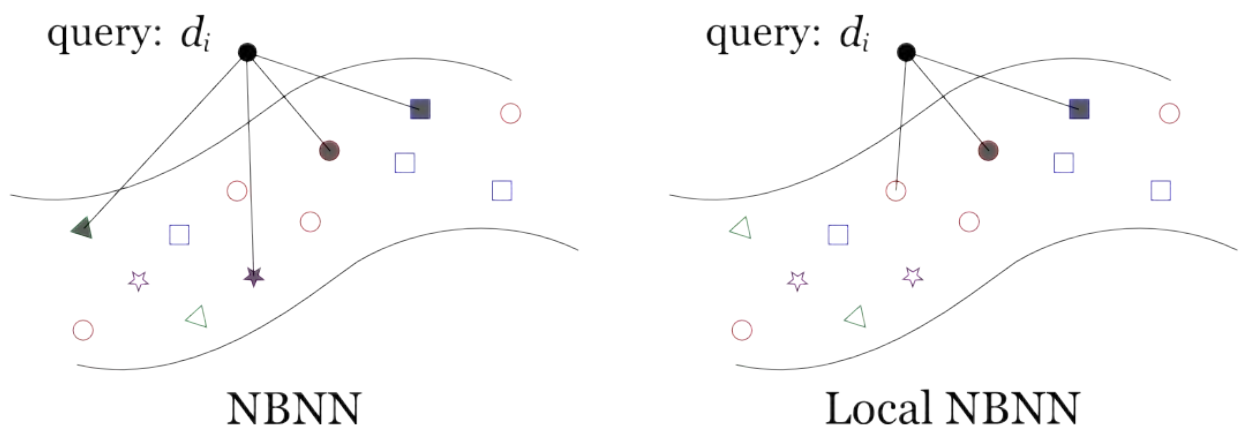
\includegraphics[width=0.6\textwidth]{images/nbnn_comp}
  \caption{NBNN vs. local NBNN \cite{mccann2012local}. NBNN looks at the nearest
  neighbours in all classes, whereas local NBNN just looks at the local region,
  regardless of what classes are present in the database.}
  \label{fig:nbnncomp}
\end{figure}

Funkhouser and Shilane present a method for querying a database of 3D objects
represented by local shape features \cite{funkhouser2006partial}. Partial
matches (correspondences) are stored in a priority queue sorted by geometric
deformation and the feature similarity. This means that only objects in the
database with a high probability of being a match need to be processed.

Some work has been done on optimising the retrieval of relevant images by
learning from user input \cite{rui2000optimizing}. When retrieved images are
presented, the user ranks them in terms of relevance, and this rank is then used
to improve the relevance of future searches.

\printbibliography
\end{document}